\documentclass[varwidth=17cm]{standalone}

\usepackage{pgfplots}
\pgfplotsset{compat=1.16}
\usepgfplotslibrary{smithchart}

% This file contains configuration shared between main file and figures

\usepackage{pifont}
\usepackage{xspace}
\DeclareUnicodeCharacter{2460}{\ding{172}\xspace}
\DeclareUnicodeCharacter{2461}{\ding{173}\xspace}

\usepackage{tikz}

\definecolor{HB9UFblue}{RGB}{0,61,165}
\definecolor{HB9UFred}{HTML}{ED135A}

\newcommand{\Ohm}{$\Omega$\xspace}


\newcommand{\uline}[1]{%
  \tikz[baseline=(todotted.base)]{
      \node[inner sep=1pt,outer sep=0pt] (todotted) {#1};
      \draw[color=HB9UFblue,thick] (todotted.south west) -- (todotted.south east);
  }%
}%
                           
\newcommand{\udash}[1]{%
  \tikz[baseline=(todotted.base)]{
      \node[inner sep=1pt,outer sep=0pt] (todotted) {#1};
      \draw[dashed,color=HB9UFred,thick] (todotted.south west) -- (todotted.south east);
  }%
}%


\begin{document}
    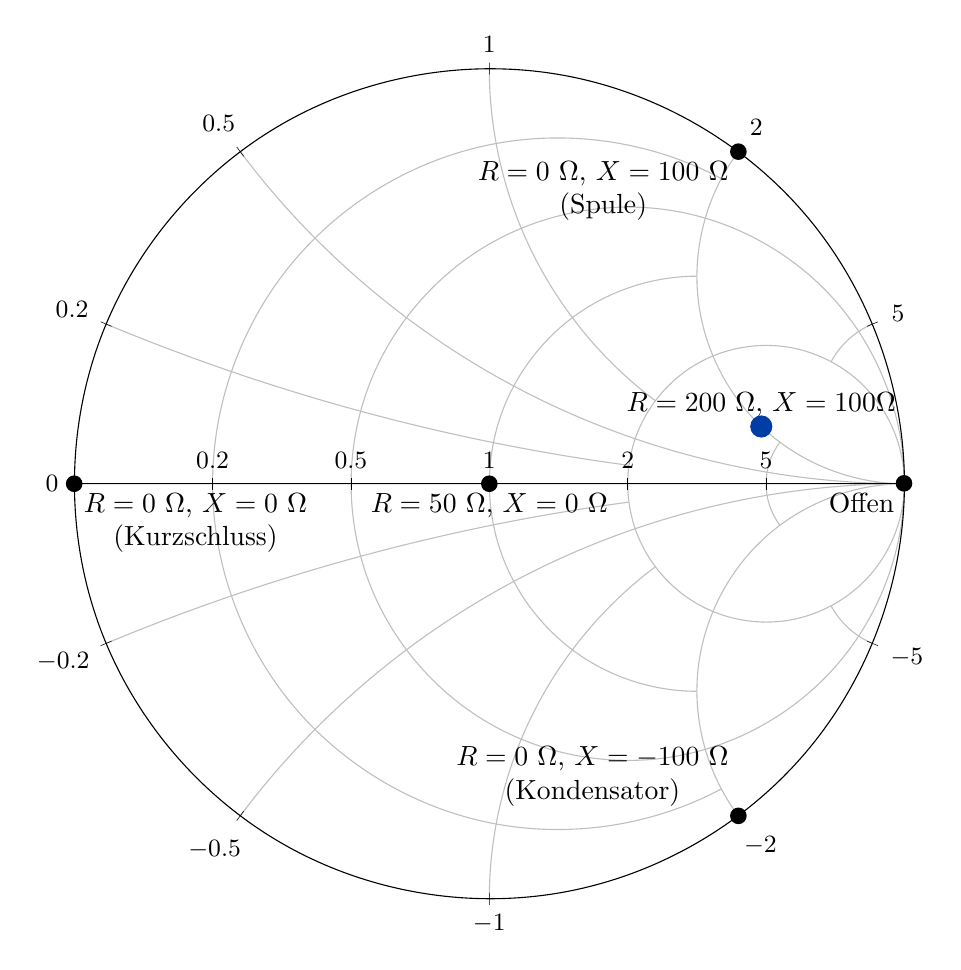
\begin{tikzpicture}
        \begin{smithchart}[width=\textwidth,show origin code/.code={},clip=false,xticklabel style={font=\small},yticklabel style={font=\small}]
            \tikzstyle{note}=[align=center,fill=black]
            \fill [note,fill=HB9UFblue] (axis cs:4,2) circle [radius=4pt] node[above] {$R=200$~\Ohm, $X=100$\Ohm};
            \fill[note] (axis cs:1,0) circle [radius=3pt] node[below] {$R=50$~\Ohm, $X=0$~\Ohm};
            \fill[note] (axis cs:0,2) circle [radius=3pt] node[below left] {$R=0$~\Ohm, $X=100$~\Ohm\\ (Spule)};
            \fill[note] (axis cs:0,-2) circle [radius=3pt] node[above left] {$R=0$~\Ohm, $X=-100$~\Ohm\\ (Kondensator)};
            \fill[note] (axis cs:0,0) circle [radius=3pt] node[below right] {$R=0$~\Ohm, $X=0$~\Ohm\\ (Kurzschluss)};
            \fill[note] (axis cs:1000,1000) circle [radius=3pt] node[below left] {Offen};
        \end{smithchart}
    \end{tikzpicture}
\end{document}
